 \section{Software}
Die Software gliedert sich in einen Teil für den Sensorprint auf dem Modul und einen Teil für den Meldeprint beim Gleichrichter. Der Teil für den Sensorprint muss unabhängig und wartungsfrei ablaufen können, wohingegen der Teil des Meldeprints in Interaktion mit dem Benutzer steht. Der Meldeprint bildet den wichtigsten Teil des Bindeglieds zwischen Benutzer und Hardware. Damit er die einzelnen Module identifizieren kann wird bei der Installation dem Sensorprints eine Identifikationsnummer gegeben. Zudem muss der Benutzer im Interface des Meldeprints die Anzahl Module angeben. Die Gemessenen Spannungswerte der Module werden via Powerline an den Meldeprint gesendet. Es sollen keine extra Datenkabel verwendet werden. Diese Daten müssen in der Meldezentrale auf dem Meldeprint verarbeitet werden. Eine allfällige Abweichung des Spannungswertes bei einem oder mehreren Modulen sollen erkannt und identifiziert werden. Worin genau diese Abweichung besteht, wird später erläutert. Nach der Identifikation muss ein solcher Fehler gemeldet werden. Die Kommunikation zwischen Hardware und Software basiert auf SPI. Das Endprodukt setzt sich aus Melde- und Sensorprint zusammen. In dieser Unterteilung werden in den nächsten Kapiteln alle Softwarekomponenten beschrieben.
\subsection{Sensorprint}
Der Sensorprint übernimmt die Spannungsmessung und sendet diese mit der Identifikationsnummer via Powerline an den Meldeprint. Die Kopplung in die Powerline gelingt mit einem Transceiver. In den Folgenden Kapiteln wird die Software weiter unterteilt und jeder Bereich einzeln erläutert.
\subsubsection{Aufbau und Abläufe (Flussdiagramm)}
\subsubsection{Inbetriebnahme}
wieso-was-wie-unter welchen Bedingungen
\subsubsection{Spannungsmessung}
wieso-was-wie-unter welchen Bedingungen
\subsubsection{Identifikation}
wieso-was-wie-unter welchen Bedingungen
\subsubsection{Transceiveransteuerung}
wieso-was-wie-unter welchen Bedingungen
\subsection{Meldeprint}
%HIER SCHREIBT CLAUDIUS
Die Software des Meldeprints ist in drei Bereiche unterteilt. Beinahe die ganze Überwachung der Module kann in einem Bereich abgehandelt werden. Die anderen beiden dienen zum einen für die Anzeige und die Initialisierung und zum anderen für die Aktualisierung der eingehenden Daten.

\begin{figure}[htbp] 
  \centering
     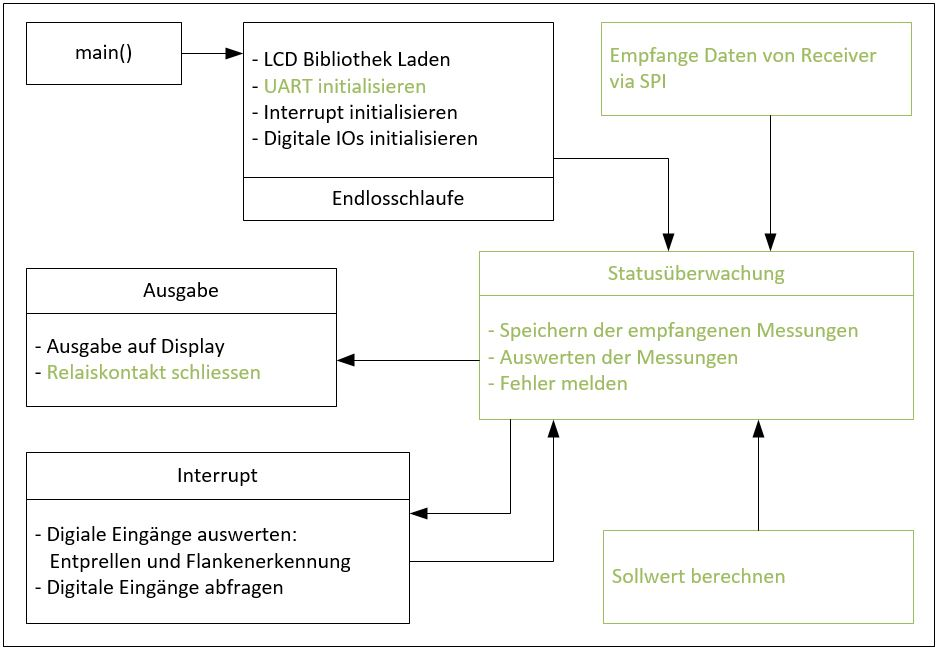
\includegraphics[width=1\textwidth]{graphics/reportboard-software-river}
  \caption{Visualisierung Softwarekonzept}
  \label{fig:reportboard-software-river}
\end{figure}

Wie die Bereiche der Software zusammenarbeiten ist in Abbildung \ref{fig:reportboard-software-river} gut ersichtlich. In der Initialisierung werden als erstes die Hardwarekomponenten und Interrupts initialisiert, dann wird die Endlosschlaufe aufgerufen.
\newline
Der initialisierte Timer Interrupt ruft dann alle 15$u$s die Routine auf, die den Receiver nach Daten abfragt und die digitalen Eingänge entprellt und eine Flankendetektion durchführt.
\newline
Die Endlosschlaufe ruft eine Routine auf, die jeweils eingegangene Daten, der gemessenen Spannung, mit der Identifikationsnummer der Sensorprints in ein Array speichert und mit dem Sollwert vergleicht. Der Sollwert entspricht dem arithmetischen Mittelwert der Spannungen dieses einen Strings von Modulen. Bei einer Abweichung von 20 Prozent, wird dasjenige Modul vorgemerkt. Falls nach einer weiteren Messung die Spannung des selben Moduls gleich vom Mittelwert abweicht, muss ein Fehler gemeldet werden. Die Identifikationsnummer wird auf dem Display angezeigt. Der ganze Prozess vom Start des Meldeprints bis zur Fehlermeldung werden hier weiter vertieft behandelt.
\todo{ich würde nach der einleitung des meldeprints keine subsection machen für das flussdiagramm}

\subsubsection{Aufbau und Abläufe (Flussdiagramm)}
\subsubsection{Inbetriebnahme}
%HIER SCHREIBT CLAUDIUS
Bei der Inbetriebnahme werden als erstes die Peripheriegeräte initialisiert. Darunter befinden sich der LCD Display und der Receiver. Weiter muss die UART Kommunikation und der Timer Interrupt initialisiert werden. In der Endlosschlaufe des Hauptprogramms werden dann die ganzen Daten der Sensorplatine gespeichert und in einem Array Register gespeichert und weiterverarbeitet.

\subsubsection{Receiver}
%HIER SCHREIBT CLAUDIUS
Der Receiver detektiert über einen Ferrit-Kern über der DC-Leitung des Strings die Signale der Sensorplatine. Die Datenpakete werden mit der Identifikationsnummer an den Arduino weitergeleitet über die UART Kommunikation.

\subsubsection{Fehlererkennung}
Aus Zeitgründen konnte die Datenverarbeitung noch nicht programmiert werden. Der Plan ist aber die gemittelten Spannungswerte, die jede Sensorplatine liefert, nochmals über alle Module des Strings zu mitteln. Damit kann dann die Standardabweichung berechnet werden. Ist die Abweichung eines Wertes mehr als 20 Prozent über der Standardabweichung, wird diese Solarmodul vorgemerkt. Diese Prozedere wiederholt sich stündlich. Weicht der Spannungswert des vorgemerkten Moduls nach der nächsten Stunde noch immer so stark vom Mittelwert ab, wird eine Fehlermeldung losgeschickt.

wieso-was-wie-unter welchen Bedingungen
\subsubsection{Fehlermeldung (Display und Relais)}
Die Fehlermeldung besteht aus der Fehlerankündigung selbst und der Identifikationsnummer der Sensorplatine, welche am defekten oder verschmutzten Modul befestigt ist. Die Fehlerankündigung ist als Text wie beispielsweise "Problem beim Modul..." auf dem Display zu sehen. Die Identifikationsnummer des Moduls wird von einer 8bit Binärzahl in eine Dezimalzahl umgewandelt und so angezeigt.

wieso-was-wie-unter welchen Bedingungen
\subsubsection{Benutzerinterface (Display und Drehgeber)}

Das Menü und der Drehgeber bilden zusammen eine einfache Schnittstelle zwischen Mensch und Maschine. Das Menü ist in drei Ebenen unterteilt welche in Abbildung \todo{Abbildung Menü} dargestellt ist.


